% GNUPLOT: LaTeX picture with Postscript
\begingroup
  \makeatletter
  \providecommand\color[2][]{%
    \GenericError{(gnuplot) \space\space\space\@spaces}{%
      Package color not loaded in conjunction with
      terminal option `colourtext'%
    }{See the gnuplot documentation for explanation.%
    }{Either use 'blacktext' in gnuplot or load the package
      color.sty in LaTeX.}%
    \renewcommand\color[2][]{}%
  }%
  \providecommand\includegraphics[2][]{%
    \GenericError{(gnuplot) \space\space\space\@spaces}{%
      Package graphicx or graphics not loaded%
    }{See the gnuplot documentation for explanation.%
    }{The gnuplot epslatex terminal needs graphicx.sty or graphics.sty.}%
    \renewcommand\includegraphics[2][]{}%
  }%
  \providecommand\rotatebox[2]{#2}%
  \@ifundefined{ifGPcolor}{%
    \newif\ifGPcolor
    \GPcolortrue
  }{}%
  \@ifundefined{ifGPblacktext}{%
    \newif\ifGPblacktext
    \GPblacktextfalse
  }{}%
  % define a \g@addto@macro without @ in the name:
  \let\gplgaddtomacro\g@addto@macro
  % define empty templates for all commands taking text:
  \gdef\gplbacktext{}%
  \gdef\gplfronttext{}%
  \makeatother
  \ifGPblacktext
    % no textcolor at all
    \def\colorrgb#1{}%
    \def\colorgray#1{}%
  \else
    % gray or color?
    \ifGPcolor
      \def\colorrgb#1{\color[rgb]{#1}}%
      \def\colorgray#1{\color[gray]{#1}}%
      \expandafter\def\csname LTw\endcsname{\color{white}}%
      \expandafter\def\csname LTb\endcsname{\color{black}}%
      \expandafter\def\csname LTa\endcsname{\color{black}}%
      \expandafter\def\csname LT0\endcsname{\color[rgb]{1,0,0}}%
      \expandafter\def\csname LT1\endcsname{\color[rgb]{0,1,0}}%
      \expandafter\def\csname LT2\endcsname{\color[rgb]{0,0,1}}%
      \expandafter\def\csname LT3\endcsname{\color[rgb]{1,0,1}}%
      \expandafter\def\csname LT4\endcsname{\color[rgb]{0,1,1}}%
      \expandafter\def\csname LT5\endcsname{\color[rgb]{1,1,0}}%
      \expandafter\def\csname LT6\endcsname{\color[rgb]{0,0,0}}%
      \expandafter\def\csname LT7\endcsname{\color[rgb]{1,0.3,0}}%
      \expandafter\def\csname LT8\endcsname{\color[rgb]{0.5,0.5,0.5}}%
    \else
      % gray
      \def\colorrgb#1{\color{black}}%
      \def\colorgray#1{\color[gray]{#1}}%
      \expandafter\def\csname LTw\endcsname{\color{white}}%
      \expandafter\def\csname LTb\endcsname{\color{black}}%
      \expandafter\def\csname LTa\endcsname{\color{black}}%
      \expandafter\def\csname LT0\endcsname{\color{black}}%
      \expandafter\def\csname LT1\endcsname{\color{black}}%
      \expandafter\def\csname LT2\endcsname{\color{black}}%
      \expandafter\def\csname LT3\endcsname{\color{black}}%
      \expandafter\def\csname LT4\endcsname{\color{black}}%
      \expandafter\def\csname LT5\endcsname{\color{black}}%
      \expandafter\def\csname LT6\endcsname{\color{black}}%
      \expandafter\def\csname LT7\endcsname{\color{black}}%
      \expandafter\def\csname LT8\endcsname{\color{black}}%
    \fi
  \fi
  \setlength{\unitlength}{0.0500bp}%
  \begin{picture}(5668.00,4534.00)%
    \gplgaddtomacro\gplbacktext{%
      \csname LTb\endcsname%
      \put(726,1050){\makebox(0,0)[r]{\strut{} 335}}%
      \csname LTb\endcsname%
      \put(726,1614){\makebox(0,0)[r]{\strut{} 340}}%
      \csname LTb\endcsname%
      \put(726,2178){\makebox(0,0)[r]{\strut{} 345}}%
      \csname LTb\endcsname%
      \put(726,2742){\makebox(0,0)[r]{\strut{} 350}}%
      \csname LTb\endcsname%
      \put(726,3306){\makebox(0,0)[r]{\strut{} 355}}%
      \csname LTb\endcsname%
      \put(726,3870){\makebox(0,0)[r]{\strut{} 360}}%
      \csname LTb\endcsname%
      \put(961,484){\makebox(0,0){\strut{} 0}}%
      \csname LTb\endcsname%
      \put(1374,484){\makebox(0,0){\strut{} 2}}%
      \csname LTb\endcsname%
      \put(1787,484){\makebox(0,0){\strut{} 4}}%
      \csname LTb\endcsname%
      \put(2200,484){\makebox(0,0){\strut{} 6}}%
      \csname LTb\endcsname%
      \put(2613,484){\makebox(0,0){\strut{} 8}}%
      \csname LTb\endcsname%
      \put(3026,484){\makebox(0,0){\strut{} 10}}%
      \put(3364,3996){\makebox(0,0)[l]{\strut{} 0.027}}%
      \put(3364,3109){\makebox(0,0)[l]{\strut{} 0.028}}%
      \put(3364,1835){\makebox(0,0)[l]{\strut{} 0.0295}}%
      \put(3364,1022){\makebox(0,0)[l]{\strut{} 0.0305}}%
      \put(220,2486){\rotatebox{-270}{\makebox(0,0){\strut{}Solvent electron density / nm$^{-3}$}}}%
      \put(4199,2486){\rotatebox{270}{\makebox(0,0){\strut{}X-ray Transmission / $\%$}}}%
      \put(2045,154){\makebox(0,0){\strut{}Vertical Position / mm}}%
    }%
    \gplgaddtomacro\gplfronttext{%
      \csname LTb\endcsname%
      \put(4729,704){\makebox(0,0)[l]{\strut{} 100}}%
      \put(4729,1213){\makebox(0,0)[l]{\strut{} 120}}%
      \put(4729,1722){\makebox(0,0)[l]{\strut{} 140}}%
      \put(4729,2231){\makebox(0,0)[l]{\strut{} 160}}%
      \put(4729,2741){\makebox(0,0)[l]{\strut{} 180}}%
      \put(4729,3250){\makebox(0,0)[l]{\strut{} 200}}%
      \put(4729,3759){\makebox(0,0)[l]{\strut{} 220}}%
      \put(4729,4269){\makebox(0,0)[l]{\strut{} 240}}%
      \put(5323,2486){\rotatebox{270}{\makebox(0,0){\strut{}Diffusion Time / min}}}%
    }%
    \gplbacktext
    \put(0,0){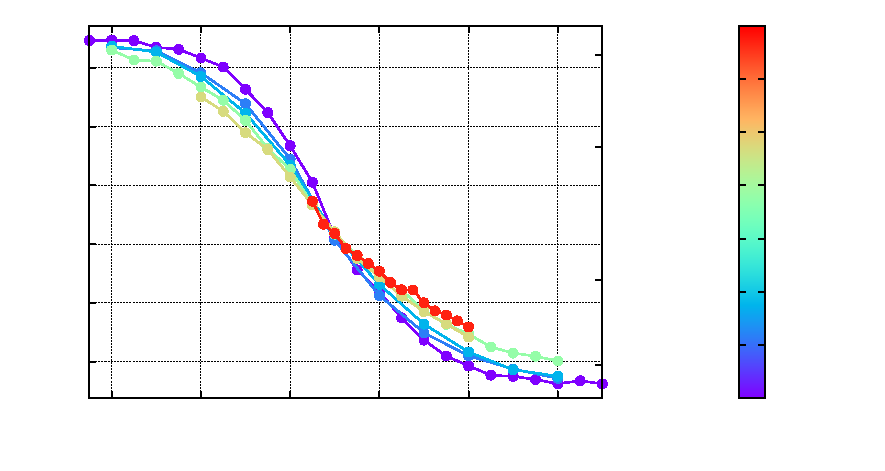
\includegraphics{KiskerTransmissionCalibration}}%
    \gplfronttext
  \end{picture}%
\endgroup
